\newpage
\section{More about Quasi Particles}
\subsection{A soluble fermion system: The pure Hartree model}
Imagine that we have an N-fermion system with no external potential, and with a pure forward-scattering interaction between particles of the form
$$V_{k l m n}=V_{k l k l} \delta_{m k} \delta_{n l}$$
Placing this in the general Hamiltonian yields
\begin{equation}H=\sum_{k} \epsilon_{k} c_{k}^{\dagger} c_{k}+\frac{1}{2} \sum_{k i} V_{k l k l} c_{l}^{\dagger} c_{k}^{\dagger} c_{k} c_{l}
\label{pure-hartree-hamil}
\end{equation}
This model H will be called the 'pure Hartree' Hamiltonian, since, as we shall show, the only terms in it are those giving rise to the 'Hartree effective field'. Our object here is to get a solution to the problem in the form of 
\begin{equation}H^{\prime}=E_{0}+\sum_{q} \epsilon_{q}^{\prime} A_{q}^{\dagger} A_{q}+\underbrace{f\left(\ldots, A_{q}, \ldots, A_{q}^{\dagger}, \ldots\right)}_{\text {small }}\end{equation}
from
\begin{equation}H=\sum_{k} \epsilon_{k} c_{k}^{\dagger} c_{k}+\frac{1}{2} \sum_{k, l, m, n} V_{k l m n} c_{l}^{\dagger} c_{k}^{\dagger} c_{m} c_{n}\end{equation},
i.e., \bluep{the ground state energy plus a set of approximately independent elementary excitations above the ground state.} We do this by the straightforward diagrammatic method.

The interaction (\ref{pure-hartree-hamil}) has only the simple forms
\begin{equation}
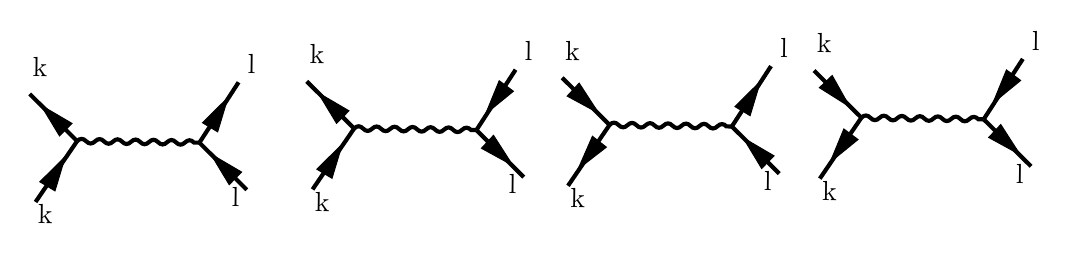
\begin{tikzpicture}[x=0.65pt,y=0.65pt,yscale=-1,xscale=1]
%uncomment if require: \path (0,705); %set diagram left start at 0, and has height of 705

%Straight Lines [id:da613823184290475] 
\draw [line width=1.5]    (69.46,540.64) .. controls (71.15,538.99) and (72.81,539.01) .. (74.46,540.7) .. controls (76.11,542.39) and (77.77,542.41) .. (79.46,540.77) .. controls (81.15,539.12) and (82.81,539.14) .. (84.46,540.83) .. controls (86.11,542.52) and (87.77,542.54) .. (89.46,540.9) .. controls (91.15,539.25) and (92.81,539.27) .. (94.46,540.96) .. controls (96.11,542.65) and (97.77,542.67) .. (99.46,541.03) .. controls (101.15,539.38) and (102.81,539.4) .. (104.46,541.09) .. controls (106.11,542.78) and (107.77,542.8) .. (109.46,541.15) .. controls (111.15,539.51) and (112.81,539.53) .. (114.46,541.22) .. controls (116.11,542.91) and (117.77,542.93) .. (119.46,541.28) .. controls (121.15,539.64) and (122.81,539.66) .. (124.45,541.35) .. controls (126.1,543.04) and (127.76,543.06) .. (129.45,541.41) .. controls (131.14,539.77) and (132.8,539.79) .. (134.45,541.48) -- (137.45,541.52) -- (137.45,541.52) ;
%Straight Lines [id:da6353755682299548] 
\draw [line width=1.5]    (43.13,514.46) -- (69.46,540.64) ;
%Straight Lines [id:da6254606220772768] 
\draw [line width=1.5]    (137.45,541.52) -- (163.78,567.69) ;
%Straight Lines [id:da5480869883300985] 
\draw [line width=1.5]    (69.46,540.64) -- (46.35,574.51) ;
%Straight Lines [id:da49445752084181116] 
\draw [line width=1.5]    (159.22,507.96) -- (137.45,541.52) ;
%Shape: Triangle [id:dp022384072825595847] 
\draw  [fill={rgb, 255:red, 0; green, 0; blue, 0 }  ,fill opacity=1 ] (49.47,520.82) -- (66.54,530.81) -- (59.69,537.75) -- cycle ;
%Shape: Triangle [id:dp5669679661948073] 
\draw  [fill={rgb, 255:red, 0; green, 0; blue, 0 }  ,fill opacity=1 ] (143.8,547.87) -- (160.86,557.87) -- (154.01,564.81) -- cycle ;
%Shape: Triangle [id:dp23872151900315752] 
\draw  [fill={rgb, 255:red, 0; green, 0; blue, 0 }  ,fill opacity=1 ] (153.28,516.53) -- (147.58,535.46) -- (139.22,530.44) -- cycle ;
%Shape: Triangle [id:dp5504301680867448] 
\draw  [fill={rgb, 255:red, 0; green, 0; blue, 0 }  ,fill opacity=1 ] (62.85,549.36) -- (57.15,568.3) -- (48.79,563.27) -- cycle ;
%Straight Lines [id:da6839577763606166] 
\draw [line width=1.5]    (223.46,533.64) .. controls (225.15,531.99) and (226.81,532.01) .. (228.46,533.7) .. controls (230.11,535.39) and (231.77,535.41) .. (233.46,533.77) .. controls (235.15,532.12) and (236.81,532.14) .. (238.46,533.83) .. controls (240.11,535.52) and (241.77,535.54) .. (243.46,533.9) .. controls (245.15,532.25) and (246.81,532.27) .. (248.46,533.96) .. controls (250.11,535.65) and (251.77,535.67) .. (253.46,534.03) .. controls (255.15,532.38) and (256.81,532.4) .. (258.46,534.09) .. controls (260.11,535.78) and (261.77,535.8) .. (263.46,534.15) .. controls (265.15,532.51) and (266.81,532.53) .. (268.46,534.22) .. controls (270.11,535.91) and (271.77,535.93) .. (273.46,534.28) .. controls (275.15,532.64) and (276.81,532.66) .. (278.45,534.35) .. controls (280.1,536.04) and (281.76,536.06) .. (283.45,534.41) .. controls (285.14,532.77) and (286.8,532.79) .. (288.45,534.48) -- (291.45,534.52) -- (291.45,534.52) ;
%Straight Lines [id:da9240174823017793] 
\draw [line width=1.5]    (197.13,507.46) -- (223.46,533.64) ;
%Straight Lines [id:da42566261374485415] 
\draw [line width=1.5]    (291.45,534.52) -- (317.78,560.69) ;
%Straight Lines [id:da016054446409110024] 
\draw [line width=1.5]    (223.46,533.64) -- (200.35,567.51) ;
%Straight Lines [id:da7774023230842375] 
\draw [line width=1.5]    (313.22,500.96) -- (291.45,534.52) ;
%Shape: Triangle [id:dp3043226594104913] 
\draw  [fill={rgb, 255:red, 0; green, 0; blue, 0 }  ,fill opacity=1 ] (203.47,513.82) -- (220.54,523.81) -- (213.69,530.75) -- cycle ;
%Shape: Triangle [id:dp9365361434860027] 
\draw  [fill={rgb, 255:red, 0; green, 0; blue, 0 }  ,fill opacity=1 ] (311.63,554.14) -- (294.29,544.63) -- (300.94,537.5) -- cycle ;
%Shape: Triangle [id:dp13172855405910544] 
\draw  [fill={rgb, 255:red, 0; green, 0; blue, 0 }  ,fill opacity=1 ] (296.64,525.44) -- (304.12,507.14) -- (311.96,512.94) -- cycle ;
%Shape: Triangle [id:dp6150273572328407] 
\draw  [fill={rgb, 255:red, 0; green, 0; blue, 0 }  ,fill opacity=1 ] (216.85,542.36) -- (211.15,561.3) -- (202.79,556.27) -- cycle ;
%Straight Lines [id:da10558670890674016] 
\draw [line width=1.5]    (505.46,527.64) .. controls (507.15,525.99) and (508.81,526.01) .. (510.46,527.7) .. controls (512.11,529.39) and (513.77,529.41) .. (515.46,527.77) .. controls (517.15,526.12) and (518.81,526.14) .. (520.46,527.83) .. controls (522.11,529.52) and (523.77,529.54) .. (525.46,527.9) .. controls (527.15,526.25) and (528.81,526.27) .. (530.46,527.96) .. controls (532.11,529.65) and (533.77,529.67) .. (535.46,528.03) .. controls (537.15,526.38) and (538.81,526.4) .. (540.46,528.09) .. controls (542.11,529.78) and (543.77,529.8) .. (545.46,528.15) .. controls (547.15,526.51) and (548.81,526.53) .. (550.46,528.22) .. controls (552.11,529.91) and (553.77,529.93) .. (555.46,528.28) .. controls (557.15,526.64) and (558.81,526.66) .. (560.45,528.35) .. controls (562.1,530.04) and (563.76,530.06) .. (565.45,528.41) .. controls (567.14,526.77) and (568.8,526.79) .. (570.45,528.48) -- (573.45,528.52) -- (573.45,528.52) ;
%Straight Lines [id:da4301121902778472] 
\draw [line width=1.5]    (479.13,501.46) -- (505.46,527.64) ;
%Straight Lines [id:da8070089193956563] 
\draw [line width=1.5]    (573.45,528.52) -- (599.78,554.69) ;
%Straight Lines [id:da9369302080120971] 
\draw [line width=1.5]    (505.46,527.64) -- (482.35,561.51) ;
%Straight Lines [id:da6514758529059829] 
\draw [line width=1.5]    (595.22,494.96) -- (573.45,528.52) ;
%Shape: Triangle [id:dp46358512529050333] 
\draw  [fill={rgb, 255:red, 0; green, 0; blue, 0 }  ,fill opacity=1 ] (498.9,521.5) -- (482.16,510.96) -- (489.23,504.24) -- cycle ;
%Shape: Triangle [id:dp38044017958960863] 
\draw  [fill={rgb, 255:red, 0; green, 0; blue, 0 }  ,fill opacity=1 ] (593.63,548.14) -- (576.29,538.63) -- (582.94,531.5) -- cycle ;
%Shape: Triangle [id:dp28303426408257704] 
\draw  [fill={rgb, 255:red, 0; green, 0; blue, 0 }  ,fill opacity=1 ] (578.64,519.44) -- (586.12,501.14) -- (593.96,506.94) -- cycle ;
%Shape: Triangle [id:dp44406046766962526] 
\draw  [fill={rgb, 255:red, 0; green, 0; blue, 0 }  ,fill opacity=1 ] (488.19,552.26) -- (495.71,533.97) -- (503.54,539.79) -- cycle ;
%Straight Lines [id:da7271479706009089] 
\draw [line width=1.5]    (365.46,531.64) .. controls (367.15,529.99) and (368.81,530.01) .. (370.46,531.7) .. controls (372.11,533.39) and (373.77,533.41) .. (375.46,531.77) .. controls (377.15,530.12) and (378.81,530.14) .. (380.46,531.83) .. controls (382.11,533.52) and (383.77,533.54) .. (385.46,531.9) .. controls (387.15,530.25) and (388.81,530.27) .. (390.46,531.96) .. controls (392.11,533.65) and (393.77,533.67) .. (395.46,532.03) .. controls (397.15,530.38) and (398.81,530.4) .. (400.46,532.09) .. controls (402.11,533.78) and (403.77,533.8) .. (405.46,532.15) .. controls (407.15,530.51) and (408.81,530.53) .. (410.46,532.22) .. controls (412.11,533.91) and (413.77,533.93) .. (415.46,532.28) .. controls (417.15,530.64) and (418.81,530.66) .. (420.45,532.35) .. controls (422.1,534.04) and (423.76,534.06) .. (425.45,532.41) .. controls (427.14,530.77) and (428.8,530.79) .. (430.45,532.48) -- (433.45,532.52) -- (433.45,532.52) ;
%Straight Lines [id:da7854992580693345] 
\draw [line width=1.5]    (339.13,505.46) -- (365.46,531.64) ;
%Straight Lines [id:da338940395062972] 
\draw [line width=1.5]    (433.45,532.52) -- (459.78,558.69) ;
%Straight Lines [id:da20114032104584845] 
\draw [line width=1.5]    (365.46,531.64) -- (342.35,565.51) ;
%Straight Lines [id:da47776944835115154] 
\draw [line width=1.5]    (455.22,498.96) -- (433.45,532.52) ;
%Shape: Triangle [id:dp9747602816540912] 
\draw  [fill={rgb, 255:red, 0; green, 0; blue, 0 }  ,fill opacity=1 ] (359.33,525.05) -- (341.95,515.63) -- (348.56,508.47) -- cycle ;
%Shape: Triangle [id:dp8973952534123313] 
\draw  [fill={rgb, 255:red, 0; green, 0; blue, 0 }  ,fill opacity=1 ] (439.8,538.87) -- (456.86,548.87) -- (450.01,555.81) -- cycle ;
%Shape: Triangle [id:dp7615505790794537] 
\draw  [fill={rgb, 255:red, 0; green, 0; blue, 0 }  ,fill opacity=1 ] (449.28,507.53) -- (443.58,526.46) -- (435.22,521.44) -- cycle ;
%Shape: Triangle [id:dp860067401387033] 
\draw  [fill={rgb, 255:red, 0; green, 0; blue, 0 }  ,fill opacity=1 ] (348.02,556.14) -- (355.95,538.02) -- (363.64,544.01) -- cycle ;

% Text Node
\draw (46.35,574.51) node [anchor=north west][inner sep=0.75pt]  [rotate=-0.74] [align=left] {k};
% Text Node
\draw (43.41,492.46) node [anchor=north west][inner sep=0.75pt]  [rotate=-0.74] [align=left] {k};
% Text Node
\draw (154.01,564.81) node [anchor=north west][inner sep=0.75pt]  [rotate=-0.74] [align=left] {l};
% Text Node
\draw (162.97,490.91) node [anchor=north west][inner sep=0.75pt]  [rotate=-0.74] [align=left] {l};
% Text Node
\draw (200.35,567.51) node [anchor=north west][inner sep=0.75pt]  [rotate=-0.74] [align=left] {k};
% Text Node
\draw (197.41,485.46) node [anchor=north west][inner sep=0.75pt]  [rotate=-0.74] [align=left] {k};
% Text Node
\draw (308.01,557.81) node [anchor=north west][inner sep=0.75pt]  [rotate=-0.74] [align=left] {l};
% Text Node
\draw (316.97,483.91) node [anchor=north west][inner sep=0.75pt]  [rotate=-0.74] [align=left] {l};
% Text Node
\draw (482.35,561.51) node [anchor=north west][inner sep=0.75pt]  [rotate=-0.74] [align=left] {k};
% Text Node
\draw (479.41,479.46) node [anchor=north west][inner sep=0.75pt]  [rotate=-0.74] [align=left] {k};
% Text Node
\draw (590.01,551.81) node [anchor=north west][inner sep=0.75pt]  [rotate=-0.74] [align=left] {l};
% Text Node
\draw (598.97,477.91) node [anchor=north west][inner sep=0.75pt]  [rotate=-0.74] [align=left] {l};
% Text Node
\draw (342.35,565.51) node [anchor=north west][inner sep=0.75pt]  [rotate=-0.74] [align=left] {k};
% Text Node
\draw (339.41,483.46) node [anchor=north west][inner sep=0.75pt]  [rotate=-0.74] [align=left] {k};
% Text Node
\draw (450.01,555.81) node [anchor=north west][inner sep=0.75pt]  [rotate=-0.74] [align=left] {l};
% Text Node
\draw (458.97,481.91) node [anchor=north west][inner sep=0.75pt]  [rotate=-0.74] [align=left] {l};


\end{tikzpicture}
\end{equation}
Hence the only graphs occurring in the series for the ground state energy are 
\begin{equation}
    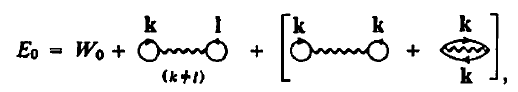
\includegraphics[width=0.8\textwidth]{screenshots/pure-hartree-diam.PNG}
    \label{pure-hartree-diam}
\end{equation}
Note that \textbf{the propagator lines in these diagrams are all hole lines. Also the diagrams in brackets violate the exclusion principle since there are simultaneously two hole lines in state $\mathbf{k}$}.
\begin{equation}E_{0}=\sum_{k<k=7} \epsilon_{k}+\frac{1}{2} \sum_{\substack{k, l<k_F\\\mathbf{k}\neq\mathbf{l}}}^{\prime} V_{k l k l}\end{equation}
The $\mathbf{k=l}$ graphs cancel because of the fermion loop in bubble diagram.

Now let us get the quasi particle energies, $\epsilon_k^{\prime}$, from the poles of the Green's function. In this case, the propagator is given exactly by the sum over just the bubble graphs:
\begin{equation}
    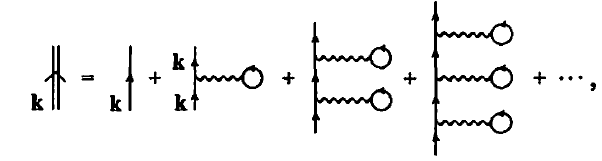
\includegraphics[width=0.8\textwidth]{screenshots/pure-hartree-diam-series.PNG}
    \label{pure-hartree-diam-series}
\end{equation}
Series (\ref{pure-hartree-diam-series}) was summed and gives the result for quasi particle energy, as shown in chapter 4,
\begin{equation}\begin{array}{l}
\epsilon_{k}^{\prime}=\epsilon_{k}+\sum_{l<k_F} V_{k l k l}, \quad k>k_{F} \\
\tau_{k}=\infty
\end{array}\end{equation}
In the case of quasi holes we just sum
\begin{equation}
    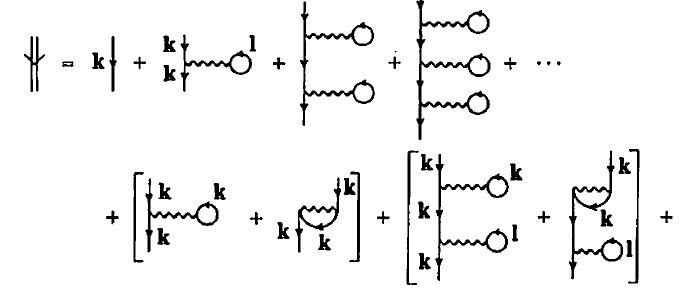
\includegraphics[width=0.8\textwidth]{screenshots/pure-hartree-hole-diam-series.PNG}
    \label{pure-hartree-hole-diam-series}
\end{equation}
The bracketed diagrams cancel because of the fermion loop and we get the result:
\begin{equation}\begin{aligned}
&\epsilon_{k}^{\prime}=\epsilon_{k}+\sum_{l<k_{F}}{}^{\prime} V_{k l k l}, \quad k<k_{F}\\
&\tau_{k}=\infty
\end{aligned}\end{equation}

Finally, we need the interaction between quasi particles ($f$-term in (\ref{pure-hartree-hamil})).This can be obtained from the various two-particle propagators. Consider the particle-particle propagator first. In the present case, this is given by the sum:
